\documentclass{scrartcl}	    % Klasse für Artikel
\usepackage[utf8]{inputenc}	% Unterstützung erweiterter Eingabe-Zeichensätze
\usepackage[ngerman]{babel}	% sprachspezifische √úbersetzungen
\usepackage[T1]{fontenc}	    % Umlaute
\usepackage{amsmath}		    % Erweiterungen für mathematischen Formelsatz
\usepackage{graphicx}        % Einbinden von Bildern
\usepackage{array}           % vertikale Ausrichtung in Tabellen
\usepackage{wrapfig}

\parindent 0mm               % kein Einzug am Absatzbeginn
\pagestyle{empty}            % keine Seitennummer

\def\uebung{10}              % Definition einer Variable (uebung)
                             % und Zuweisung eines Wertes (10)

\begin{document}

\begin{table}[h]\Large
\begin{center}
\begin{tabular}{|c|m{11.5cm}|c|}
\hline
EP\&P
&
Übungen Programmierung\newline
Dr. J. Brose, PHY C116, Tel. 32104\newline
J.Brose@physik.tu-dresden.de
&
\uebung
\\
\hline
\end{tabular}
\end{center}
\end{table}
               % Einbinden eines weiteren Dokuments

\section*{Numerische Nullstellensuche: Keplerproblem}
\emph{Die Bahnen der Planeten um die Sonne sind Ellipsen, in deren einem Brennpunkt die Sonne steht.}

Dieser einfache Sachverhalt führt zu einem analytisch nicht lösbaren Problem, wenn man versucht im System der Sonne, den Betrag des Ortsvektors $\vec{r}$(t) oder auch den Winkel $\phi$(t) des Planeten relativ zur Sonne im Zeitverlauf zu berechnen.

\begin{wrapfigure}{l}{0.5\textwidth}
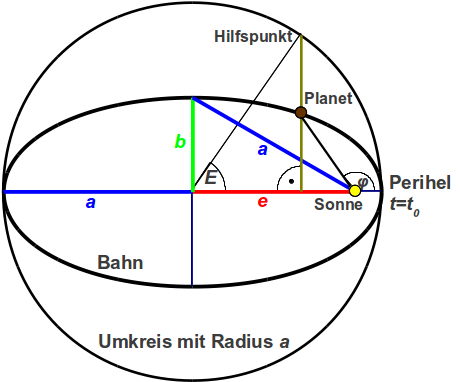
\includegraphics[width=0.48\textwidth]{Kepler_Schema.png}
\end{wrapfigure}

Die Orts- Zeitfunktion r(t) lässt sich über
die Zeitabhängigkeit der \textbf{wahren Anomalie
$\boldsymbol{\phi}$(t)} berechnen, wobei $\boldsymbol{\phi}$\textbf{(t)} der Winkel zwischen der Verbindungslinie Sonne - Perihel und der Linie Sonne - Planet ist.
\[
\mathbf{ r = r(\boldsymbol{\phi} (t)) = r(t) = a \cdot \frac{1-\boldsymbol{\epsilon}^2}{1+\boldsymbol{\epsilon} cos \boldsymbol{\phi}}}
\]

mit

\begin{description}
\item $\boldsymbol{\phi}$ -- wahre Anommalie
\item $\boldsymbol{\epsilon}$ -- numerische Exzentrität
\item $\boldsymbol{\epsilon}$ = $\frac{e}{a} = \sqrt{1-{(\frac{b}{a})}^2}$
\item \textbf{e} -- lineare Exzentrizität
\item \textbf{e} = $\sqrt{a^2 - b^2}$
\item \textbf{a} -- große Halbachse der Bahn-Ellipse
\item \textbf{b} -- kleine Halbachse der Bahn-Ellipse
\end{description}
Die wahre Anomalie ist berechenbar aus der \textbf{exzentrischen Anomalie E} (Winkel vom Mittelpunkt der Ellipse zu einem Hilfspunkt auf dem Umkreis mit Radius der großen Halbachse (Projektion des Planetenortes auf den Umkreis) relativ zur Verbindungslinie Mittelpunkt - Perihel)

\[
\phi = \underbrace{2\pi - \underbrace{arccos(\frac{cos E-\epsilon}{1-\epsilon cos E})}_{0 \le E \le \pi}}_{\pi \le E \le 2\pi}
\]


\end{document}
